\documentclass[10pt,onecolumn,journal,draftclsnofoot]{IEEEtran}
\usepackage[margin=0.75in]{geometry}
\usepackage{listings}
\usepackage{color}
\usepackage{longtable}
\usepackage{graphicx}
\usepackage{float}
\usepackage{tabu}
\usepackage{enumitem}
\usepackage{courier}
\usepackage{hyperref}
\usepackage{parskip}
\definecolor{dkgreen}{rgb}{0,0.6,0}
\definecolor{gray}{rgb}{0.5,0.5,0.5}
\definecolor{mauve}{rgb}{0.58,0,0.82}

\graphicspath{{images/}}

\lstset{frame=none,
language=C,
columns=flexible,
numberstyle=\tiny\color{gray},
keywordstyle=\color{blue},
commentstyle=\color{dkgreen},
stringstyle=\color{mauve},
breaklines=true,
breakatwhitespace=true,
tabsize=4,
showstringspaces=false,
basicstyle=\ttfamily
}

\setlength{\parindent}{0cm}

\begin{document}
\begin{titlepage}
  \pagenumbering{gobble}
  \title{POWER8 Continuous Integration\\ Winter Midterm Progress Report}
  \author{Leon Leighton, Thomas Olson, Derek Wong\\Project 35}
  \date{February 17, 2017}
  \maketitle
  \vspace{4cm}
  \begin{abstract}
  \noindent This document contains an overview of the Winter midterm progress of the POWER8 Continuous Integration project.
    It includes the goals and purpose of the project and a reflection on the previous six weeks.
 \end{abstract}
\end{titlepage}

\pagenumbering{arabic}
\tableofcontents
\clearpage

\section{Project Goals}
The primary goal of this project is to create a continuous integration (CI) system for IBM's POWER8 architecture.
This CI system will be available to open source software projects, giving them the ability to build and test their software on POWER8 without the need for them to acquire new hardware.
We will be utilizing the OSU Open Source Lab's POWER8 OpenStack cluster to deploy our project and run the builds and tests.
We also aim to make the system easy to use while still giving users the ability to customize their build environment.
Our focus will be on interacting with GitHub to trigger new builds as developers commit new changes to their code, with support for other version control systems as a stretch goal.
Users will be able to access the status of their builds to gain information about build or test failures.
They will also be able to download the binaries built by the system.
Our project will also be open source and hosted on GitHub which will allow others to replicate our project on their own systems.

\section{Fall Term Progress}
Over the Fall term we made progress in learning to work with our client, IBM, and we learned more about the various pieces of our project.
We were in regular contact with IBM with a conference call every two weeks where we discussed the project and what we had been working on.
We also had regular email exchanges with our primary contact at IBM, Gerrit Huizenga.
These email exchanges were helpful in increasing our understanding of the goals and purpose of the project and he provided valuable feedback on our documents.
We were also in contact with the OSL director, Lance Albertson, discussing access to the POWER8 OpenStack cluster.
\\
\\
Through writing the documents for Fall term, particularly the technical review and the design document, we gained knowledge about the individual components that will make up the completed CI system.
The technical review allowed us to compare alternatives which is something that will continue as we progress through the next stages of the project.
Writing the design document enabled us to start thinking about how the various pieces will work together to accomplish our goals.
In particular, we learned about Jenkins and various Jenkins plugins.
Jenkins is automation software that will be at the center of coordinating the builds and tests.
Several plugins for Jenkins exist that will allow us to interact with OpenStack and GitHub.
Writing these documents enabled us to put together ideas about how we will go forward during Winter term to implement the system.

\section{Current Progress}
The following is the status of our project as of the sixth week of Winter term. It is separated into individual team member sections.
\subsection{Leon Leighton}
I started out the term by establishing the foundation for our project.
We require a virtual machine running on the OSL's POWER8 OpenStack cluster.
This VM is where Jenkins will run and where interactions with the OpenStack cluster will originate.
I created the VM named power8ci through the OSL's OpenStack Dashboard.
Since this VM is serving as our test platform, I choose to use a smaller instance than what we may use in the future.
The power8ci VM is running Ubuntu 16.04 LE and has 2GB of RAM, 20GB of disk space, 1 VCPU, and a publicly accessible IP address.
Below is a screenshot of the OpenStack Dashboard showing our VM\@.


\begin{figure}[H]
  \centering
  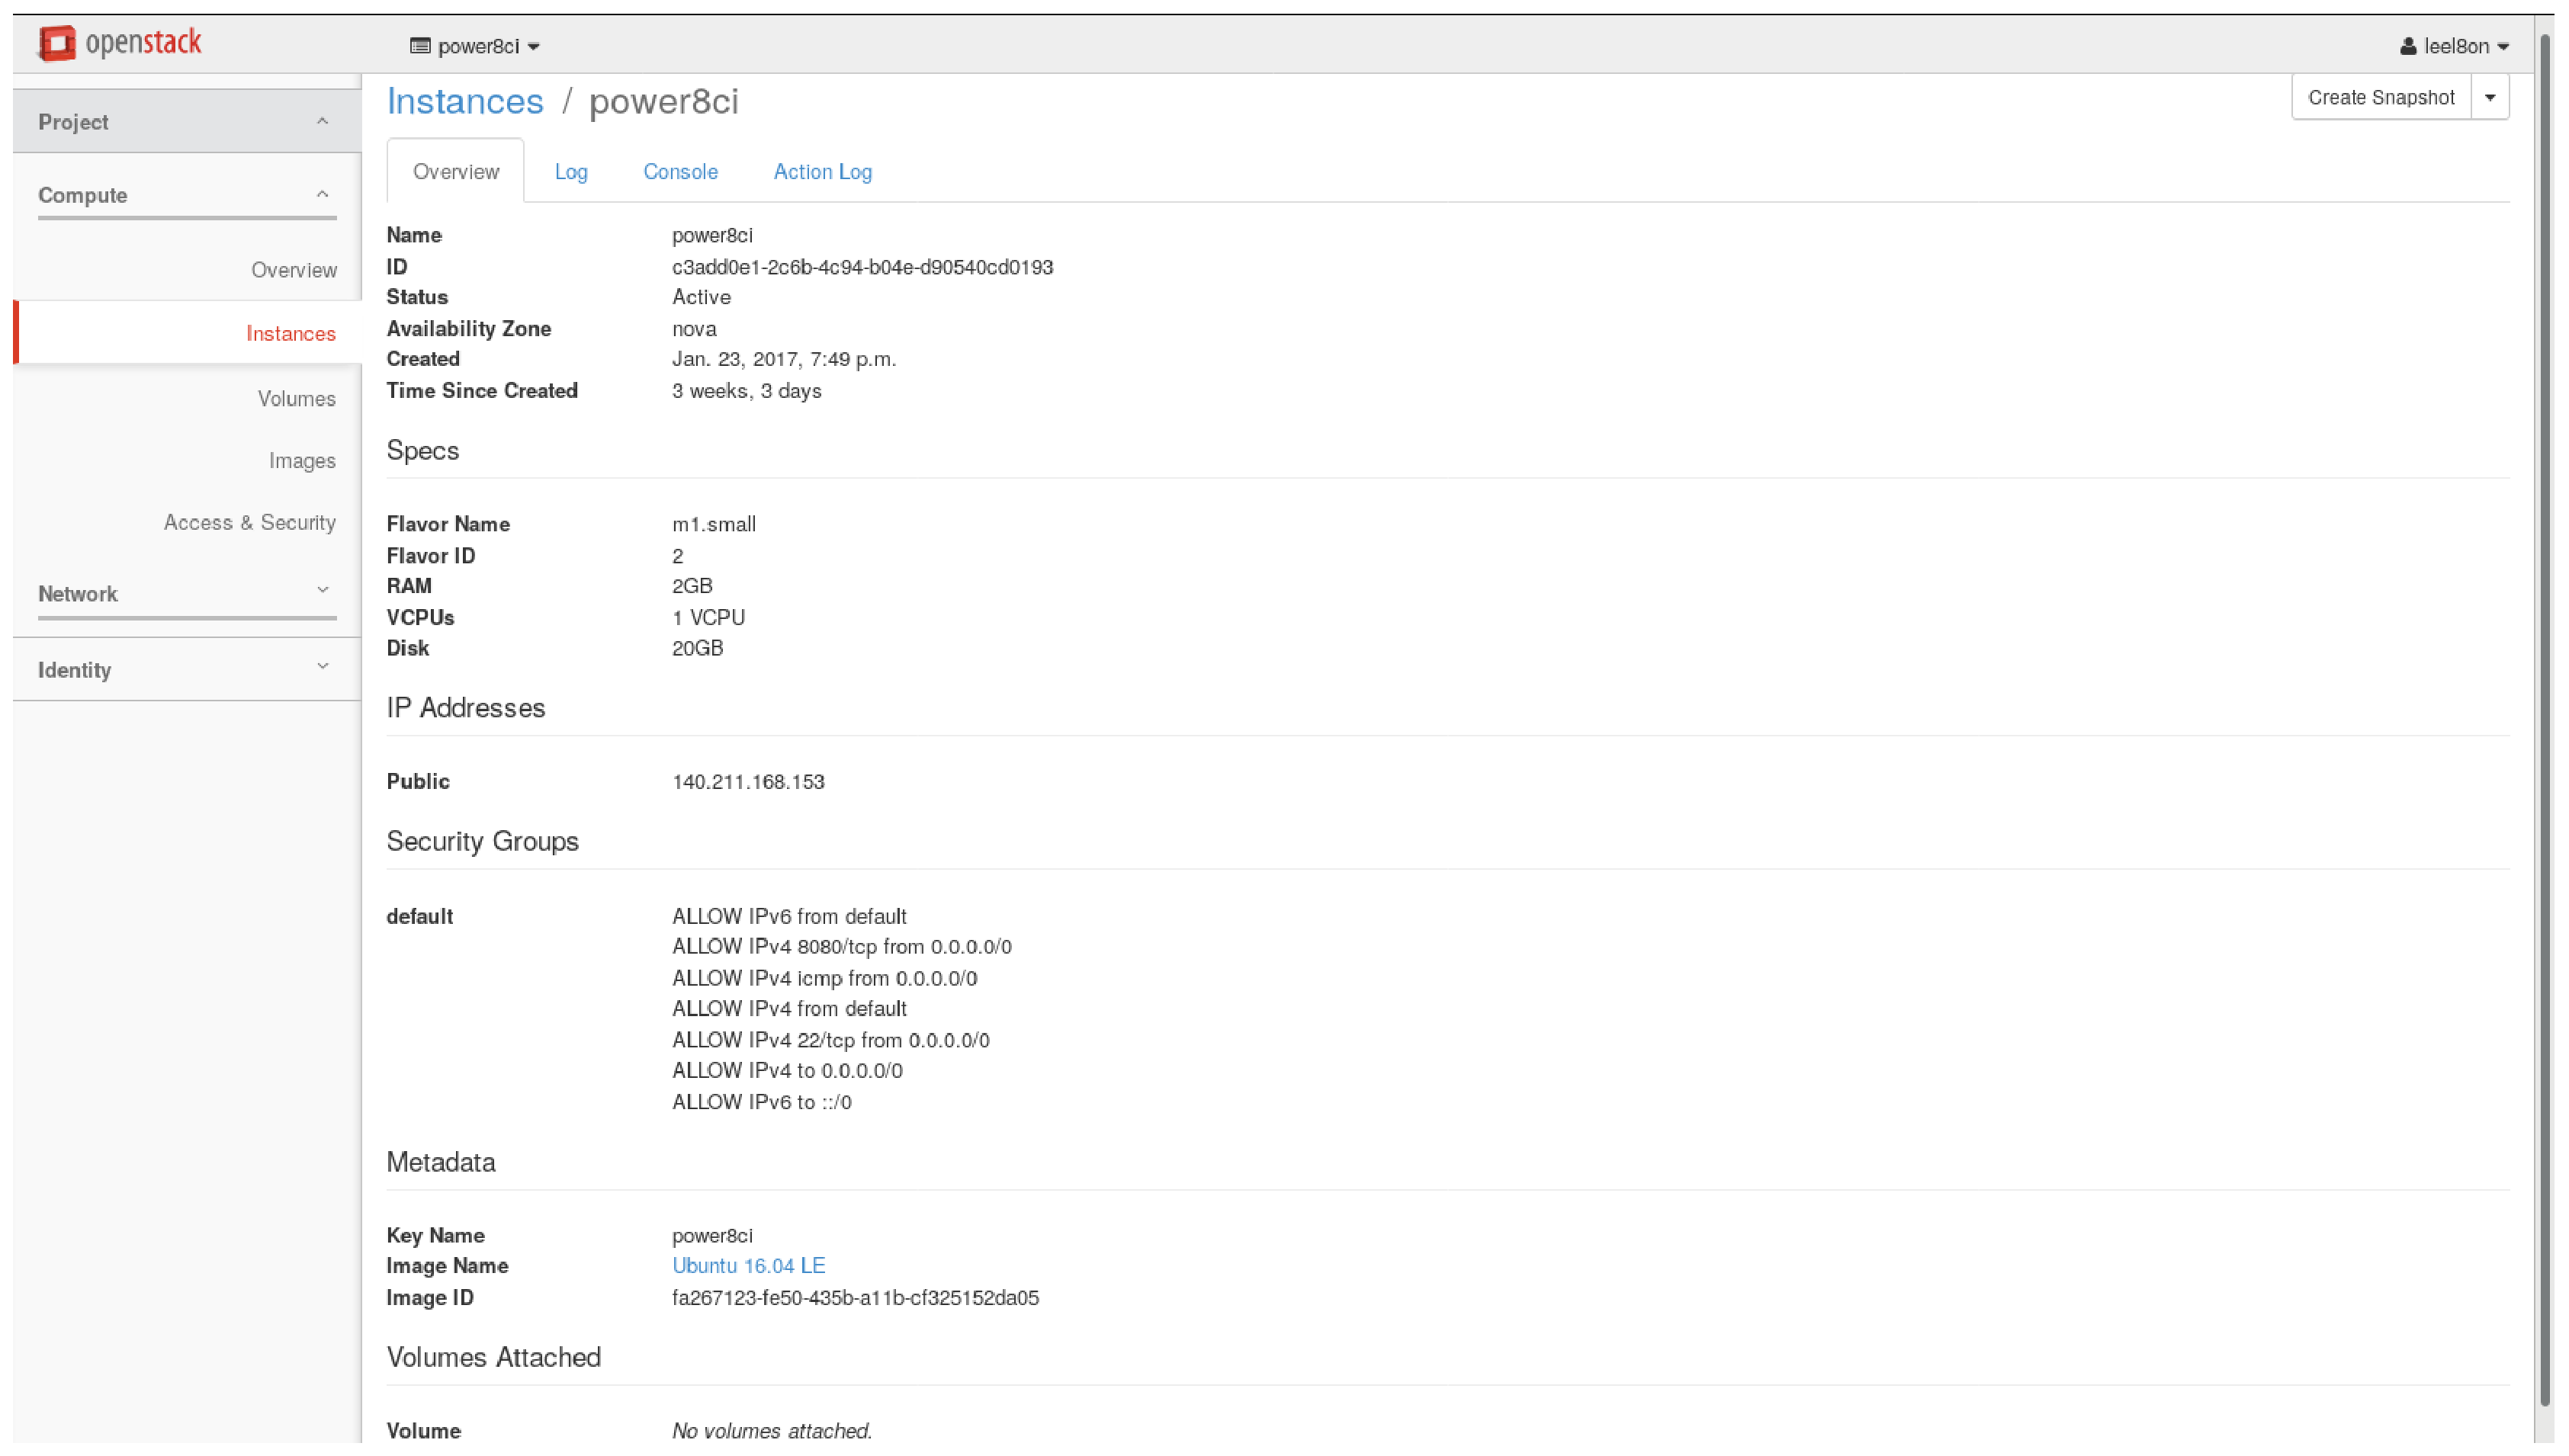
\includegraphics[width=\textwidth, keepaspectratio]{openstack.eps}
  \caption{OpenStack Dashboard showing power8ci VM}
\end{figure}

After establishing the VM, I focused on installing Jenkins using Ansible.
Ansible provides a service called Ansible Galaxy where roles can be shared with the Ansible community.
I found a role called `geerlingguy.jenkins' that installs Jenkins and its dependencies.
This role also allows options to be passed, such as which plugins to install.
After successfully running Ansible to install Jenkins, and after Derek Wong used the options to install the needed GitHub plugins,
I configured Jenkins authenticate users with their GitHub credentials.
We then created some simple jobs within Jenkins to verify its ability to pull a repository from GitHub and build the software.
We created one job that we expected to succeed and one that we expected to fail.
Both of these were very simple C programs.
We received the expected response from Jenkins in both cases.
In addition, we were able to trigger new builds by pushing a commit to GitHub.
Below is a screenshot showing our Jenkins jobs.
\begin{figure}[H]
  \centering
  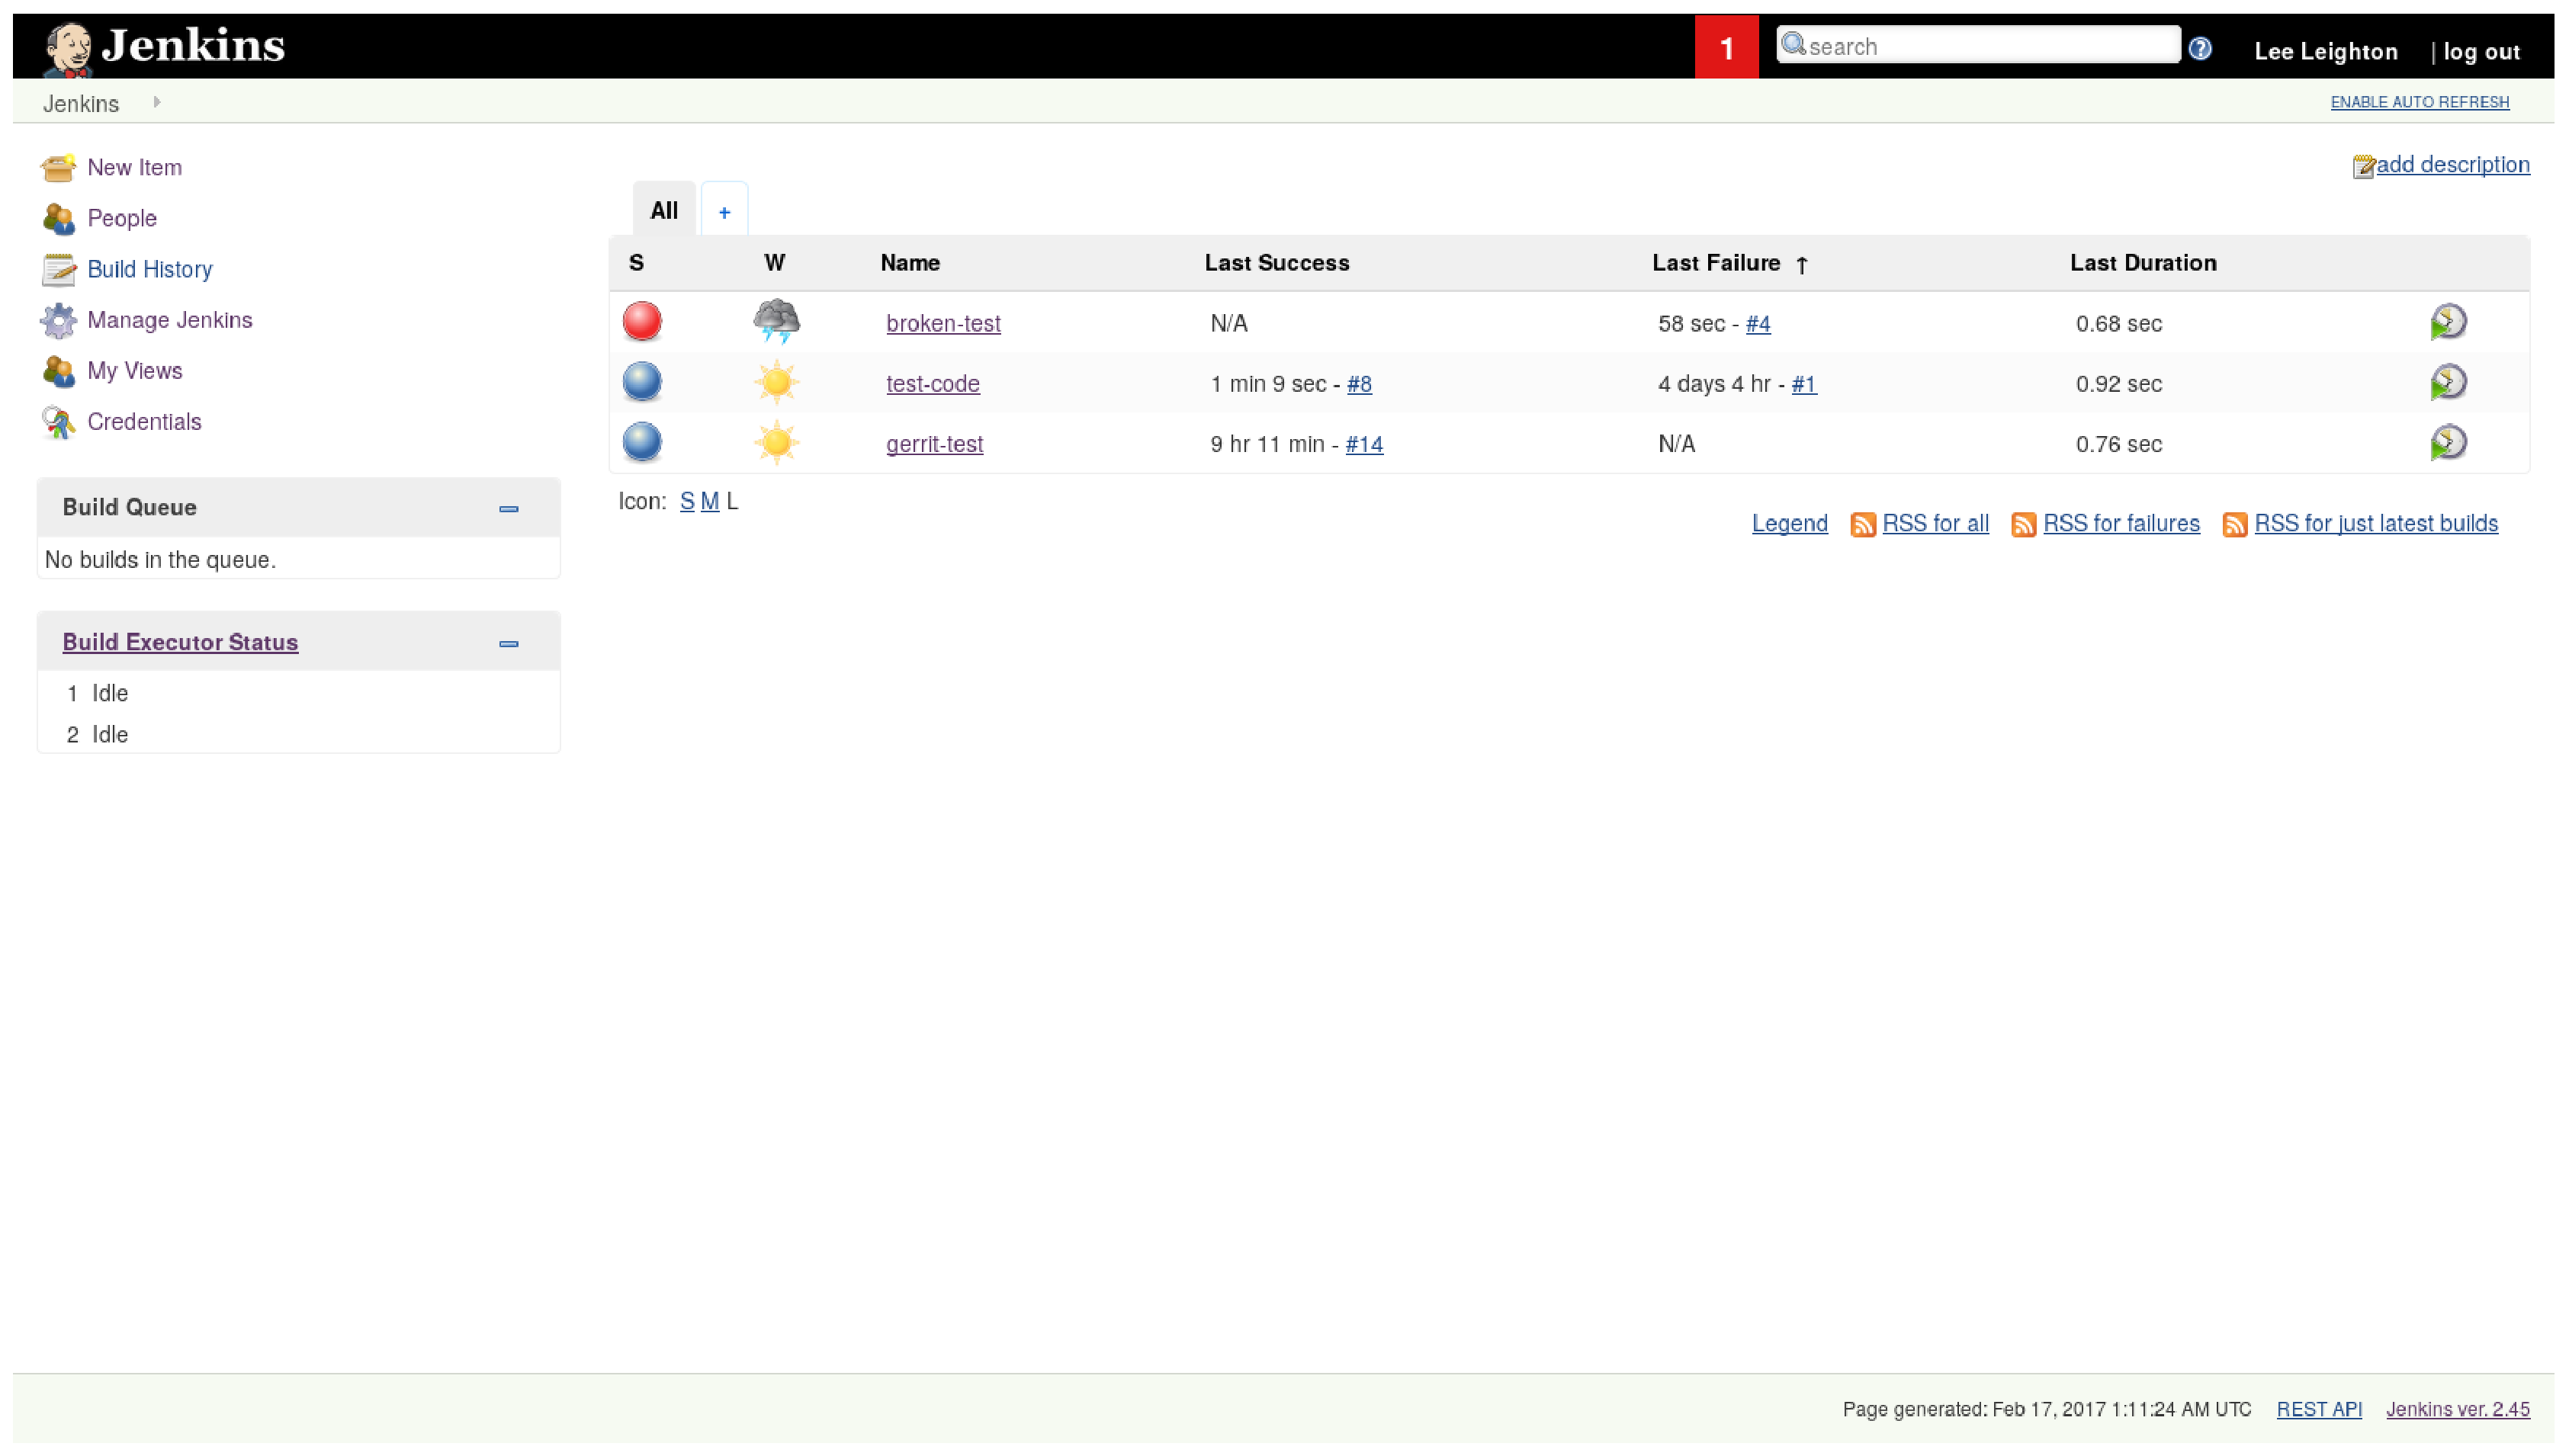
\includegraphics[width=\textwidth, keepaspectratio]{jenkins.eps}
  \caption{Jenkins job status}
\end{figure}

\subsection{Thomas Olson}
I created some diagrams to better lay out the structure of the system that we're building. I looked into the use of Docker and Kubernetes as container management solutions on a cluster. I researched methods for having Jenkins communicate with Docker, Kubernetes and Openstack to facilitate the provisioning of containers and virtual machines for running builds on. I did not do much in the form of implementation as such features would be a part of the beta release at the earliest, and not the alpha release.

\begin{figure}[H]
  \centering
  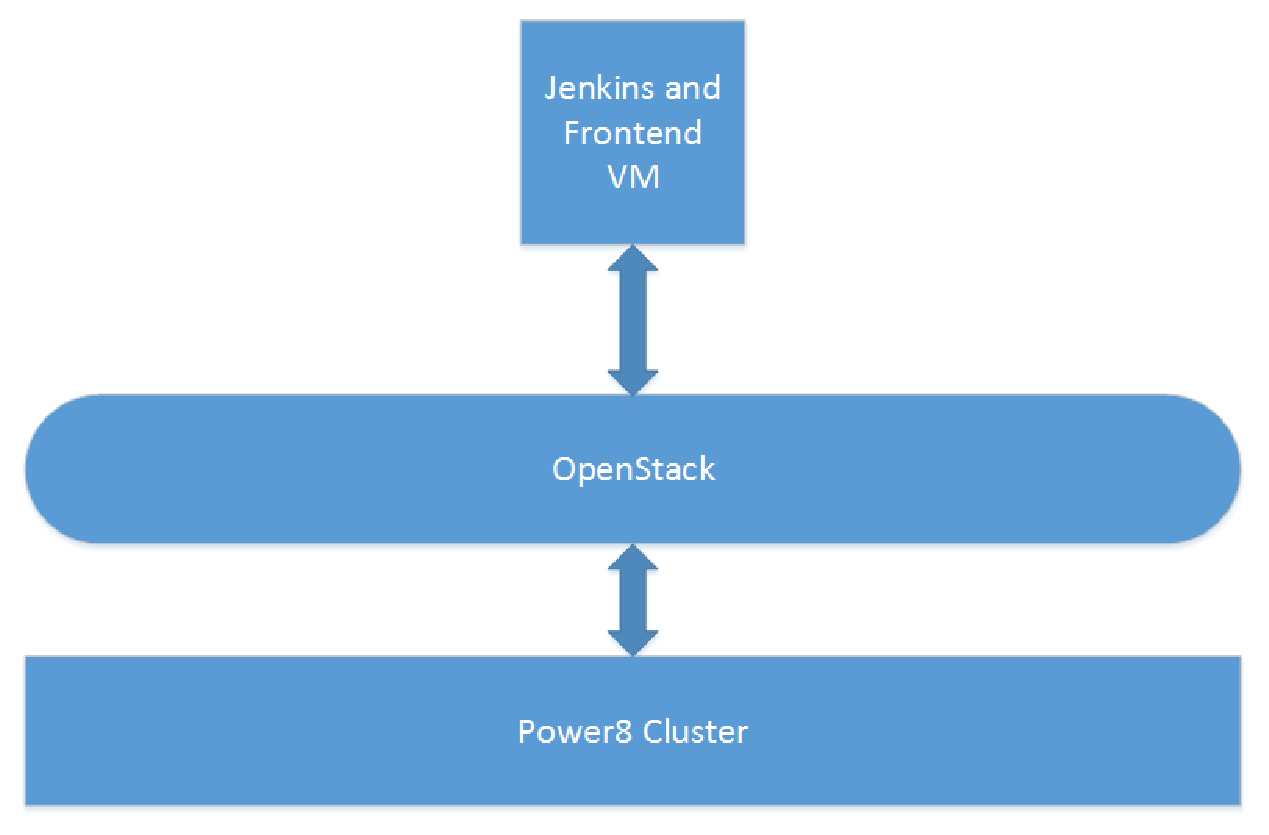
\includegraphics[width=\textwidth, keepaspectratio]{Current_Infrastructure.eps}
  \caption{Current Infrastructure}
\end{figure}
\subsection{Derek Wong}
I am mainly in charge of the plugins for our POWER8 continuous integration project. In the technology review document my focus was the login/authentication for our services and plugins that benefits our users. After Lee set up the basics of jenkins, I helped him set up the login/authentication portion of our service. In the technology review document I have decided to use the Github OAuth Plugin which uses the github account credentials to login into our services. I chose this plugin because most of our users will mainly be using github repository for their projects, so it is only logical to just let them use their github user accounts.



\section{Future Work}
\subsection{Leon Leighton}
For the rest of the term, I will be focusing on improving our Ansible playbook and integration with OpenStack.
For our solution to be reproducible, the configuration needs to be fully in Ansible.
Our current Alpha release has some configuration that has been done through the Jenkins interface.
These configuration changes will be moved into our Ansible playbook.

Our Alpha release is running on the OSL's POWER8 OpenStack cluster and all Jenkins jobs run on this one VM\@.
Moving forward, we will be introducing the ability for a Jenkins job to be run on a separate VM and/or run in a Docker container.
This will provide better isolation between Jenkins jobs.
Jenkins has an OpenStack plugin, and I will be investigating how to use it to best achieve our goals.

\subsection{Thomas Olson}
For the future, I will need to implement the system we choose to use for managing and provisioning containers and implementing a method for users to include a YAML file for configuring their build process and environment. I will also need to look into creating basic images for containers that can be used to run builds in. Finally, I will need to put all of this into the Ansible playbook so that others may deploy this part of the system on their own clusters.

\begin{figure}[H]
  \centering
  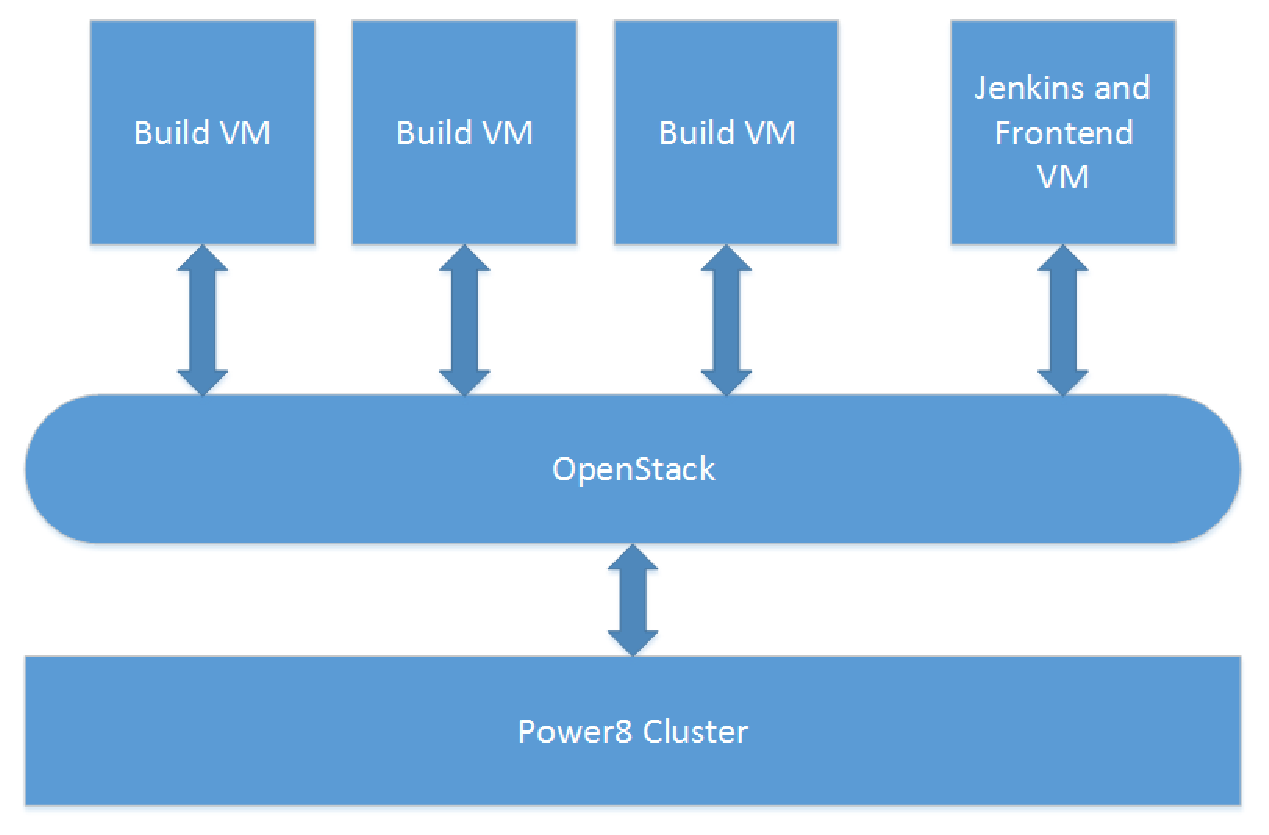
\includegraphics[width=\textwidth, keepaspectratio]{Infrastructure.eps}
  \caption{Future Infrastructure}
\end{figure}

\subsection{Derek Wong}
Now that we have basic jenkins set up, we can continue working on the configurations and making improvements to it. My job will be deciding which plugins will be necessary in our continuous integration service. I have already implemented the Github OAuth Plugin to jenkins. This plugin is used for authentication and authorization. It is what we are using to set permissions for users of our service. The next plugin that I am planning to implement is the Build Monitor Plugin, which shows all the information of a project being build, as well as unique features that benefits our users. This is one of the technology in the technology review document that we decided to use and we intend to implement it before we work on other features. As of now, those are all the plugins we are going to use, and I will continue to do more research and see what other plugins will improve and benefit our project. Aside from plugins, I will begin researching more information about security. Our client has emphasized how security is really important in our project, so that is one of the top priorities we need to do. Aside from those tasks, I will help with finding solutions to problems that we might run into in the future.


\section{Problems}
\subsection{Leon Leighton}
Unfortunately, it took longer than expected to setup and the VM and Jenkins.
This caused a problem for Thomas Olson and Derek Wong, as they could not continue some of their work until I had completed the foundational elements.

\subsection{Thomas Olson}

\subsection{Derek Wong}
The authentication for the Github OAuth Plugin works fine as it lets user login with their github credentials. We have tested it on several accounts and there were no problems. The authorization part of this plugin is a little different. Currently, it does not grant users that have permission to build a project even thought they are supposed to. We set the permissions so that users who have contributed to a project in the github repository should have the ability to create a job for that project in jenkins, and have the ability to build it. There is no solution to it currently but we are looking into it.

\end{document}
